\section{Experiments}

This section presents an evaluation of the proposed control system. Firstly, simulation results are shown to be subsequently compared to those of real-world experiments. We tested the system on various situation including tracking constant reference, step response and sine trajectory. Another experiments were conducted to verify the disturbance rejection feature. This section also includes observations of the position drift of the estimator with an absolute localization system. Finally the system's performance is compared to the previous work. Most of experiments are captured in the compilation video \url{http://youtu.be/lPy7w-GUbw4} which is also located on the enclosed CD. 

\subsection{Simulating MPC}

Figure \ref{fig:simulation_step_no_governor} shows the step response of the system, simulated without the input governor. The proaction can be seen before the step in the reference trajectory which is thanks to the predictive nature of the controller. 

\begin{figure}[H]
\centering
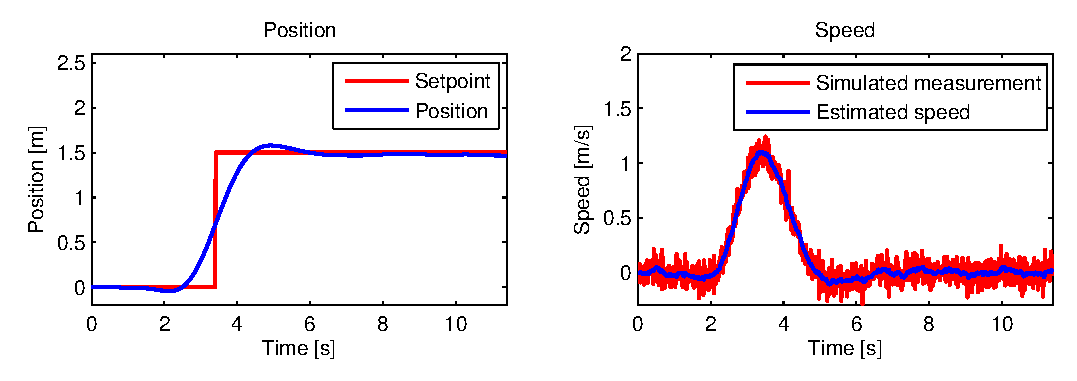
\includegraphics[width=0.99\textwidth]{fig/simulation1_step_no_governor.eps}
\caption{Simulating position step response without the input governor (forward motion).}
\label{fig:simulation_step_no_governor}
\end{figure}

\begin{figure}[H]
\centering
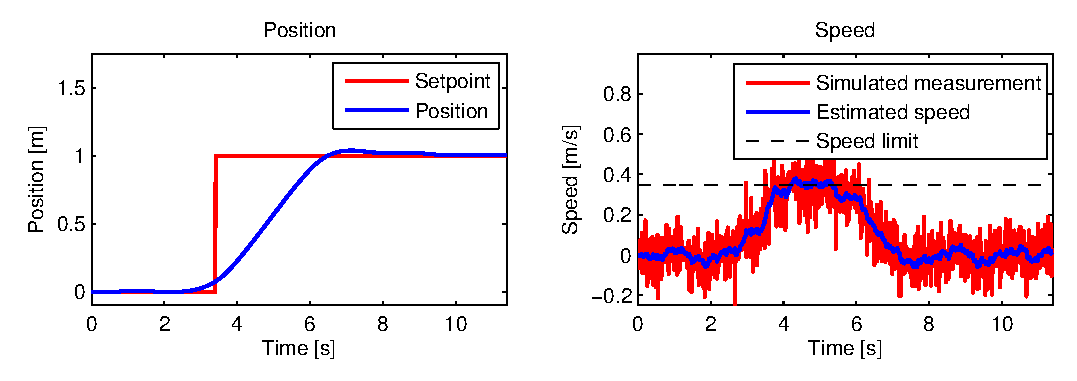
\includegraphics[width=0.99\textwidth]{fig/simulation2_step_governor.eps}
\caption{Simulating position step response with the input governor (forward motion).}
\label{fig:simulation_step_governor}
\end{figure}

Since the desired \emph{unit step} trajectory is not feasible, it should be firstly transformed using the input governor. In our case, we limit the UAV's speed to $0.35\jed{ms^{-1}}$ (which is due to maximum speed that the \emph{px4flow} sensor can reliably measure). Figure \ref{fig:simulation_step_governor} shows the Simulation of step response with the input governor. See that the speed lies roughly under the limit. Figure \ref{fig:simulation_sine} shows the simulation of UAV tracking sine trajectory. Prior work \citep{baca2013, endrych2014} and related work \citep{bangura2014realtimempc} demonstrated that tracking such trajectory is difficult without a notable lag. Our simulation shows that MPC with long enough prediction horizon should perform better. See section \ref{cap:dynamic_trajectory_tracking} for experimental validation of the trajectory.

\begin{figure}[H]
\centering
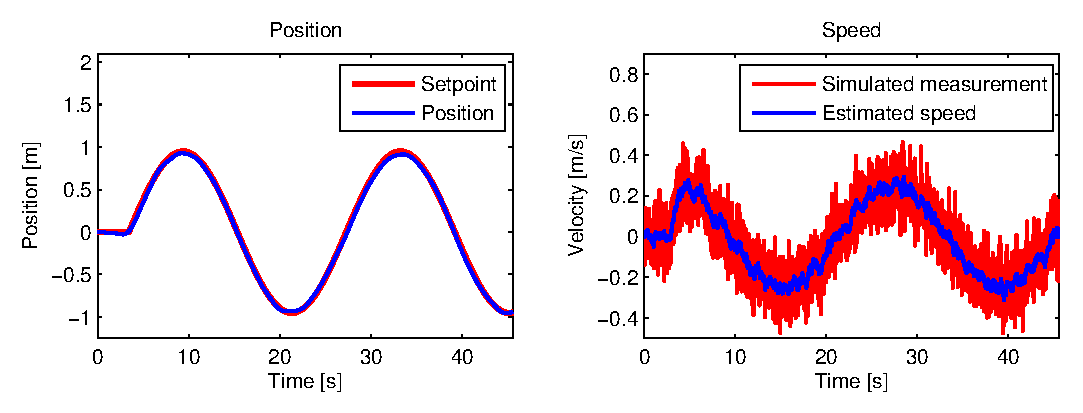
\includegraphics[width=0.99\textwidth]{fig/simulation3_sine.eps}
\caption{Simulating trajectory of feasible sine trajectory (forward motion).}
\label{fig:simulation_sine}
\end{figure}

The disturbance rejection feature based on the disturbance estimation is one of selling points of the system. It should be able to deal with constant disturbances (cause by bad trimming, offset in \emph{KK2} stabilization) as well as momentary disturbances (possibly caused by wind). Although simulations showed that the the disturbance estimation can be tuned arbitrarily to match a desired settling time of the estimation, in practice, there is a limit (see discussion in section \ref{cap:persistant_wind_disturbances_experiment}). Figure \ref{fig:simulation_disturbance_rejection} shows a simulation of the disturbance rejection with parameters tuned on the real UAV.

\begin{figure}[H]
\centering
\includegraphics[width=0.99\textwidth]{fig/simulation4_disturbance_rejection.eps}
\caption{Simulating of disturbance rejection (forward motion).}
\label{fig:simulation_disturbance_rejection}
\end{figure}

\subsection{Tracking constant setpoint}

The first experiment was to test the UAV's capability of tracking the constant reference, i.e. hovering above one place. Statistically, we are interested in the standard deviation $\sigma$ and the maximum deviation $\Delta_{max}$. Figure \ref{fig:experiment_constant_trajectory} shows its performance in good light conditions with no wind disturbances. The aircraft was capable of tracking the reference with standard deviation $\sigma = 4.8\jed{cm}$ and maximum deviation $\Delta_{max} = 14.4\jed{cm}$.

\begin{figure}[H]
\centering
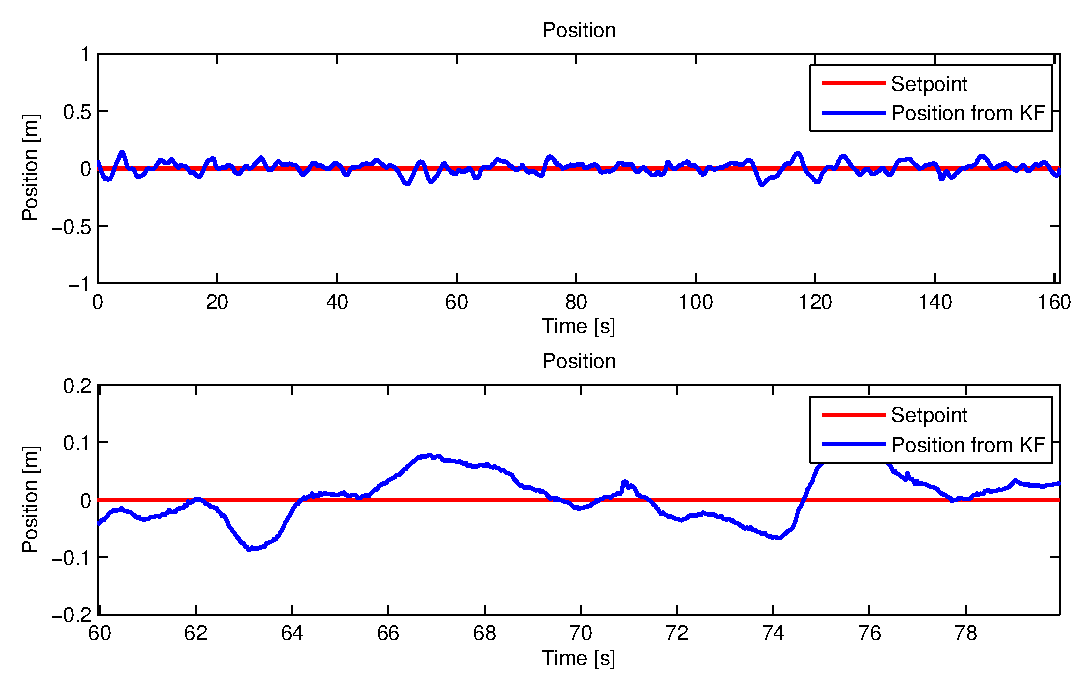
\includegraphics[width=0.99\textwidth]{fig/experiment6_constant_reference.eps}
\caption{Experiment with tracking static trajectory (forward motion).}
\label{fig:experiment_constant_trajectory}
\end{figure}

\subsection{Measuring of estimation drift}

One could ask, what is the relevance of previously presented data, since the position is estimated onboard using only velocity data and the model. The truth is, that the position is not absolute and although the controller seems to stay around the setpoint, the absolute position in the space may drift away. In order to measure such drift we implemented the Whycon camera localization system \citep{faigl2013whycon} using calibrated camera. It was used to measure the absolute position of the UAV while conduction a flight. The figure \ref{fig:experiment_drift_constant} shows the position drift during 1 minute flight. The maximum measured deviation was $\approx 10\jed{cm}$. It can be seen, that the estimated position slowly drifts away from the absolute one, and then lately drifts back. Similar effect can be observed on figure \ref{fig:experiment_drift_sine} where the UAV is tracking a sine trajectory. In general, the drift is larger when the UAV is moving closer to \emph{px4flow's} saturation.

\begin{figure}[H]
\centering
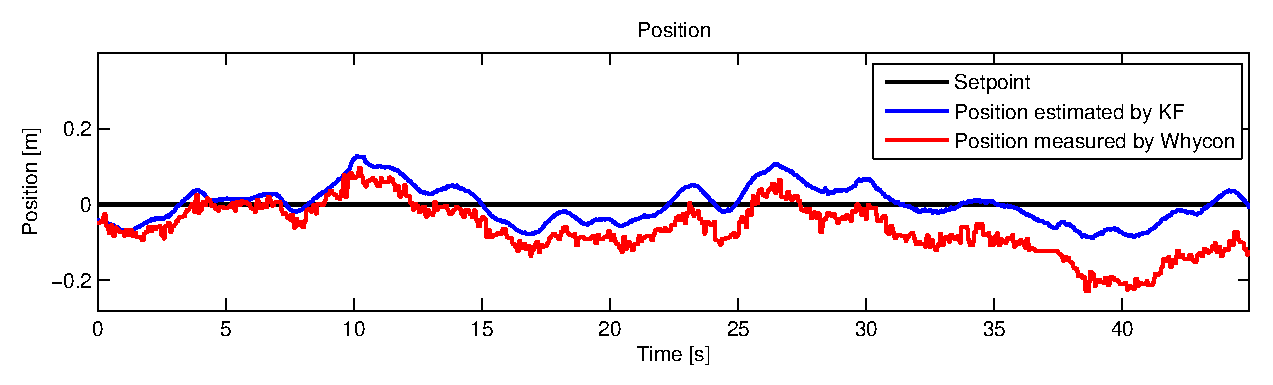
\includegraphics[width=0.99\textwidth]{fig/experiment5_drift_constant.eps}
\caption{Experiment with measuring a position drift (forward motion).}
\label{fig:experiment_drift_constant}
\end{figure}

The signal noise from \emph{px4flow} is usually larger at higher velocities. Finally, there are other conditions that need to be met to eliminate the position drift --- good light conditions and good vibration isolation of the sensor. Otherwise the drift is $\approx 10\jed{cm/min}$ or larger. Our observations correspond to those of creators of the sensor \citep{honegger2013open}.

\begin{figure}[H]
\centering
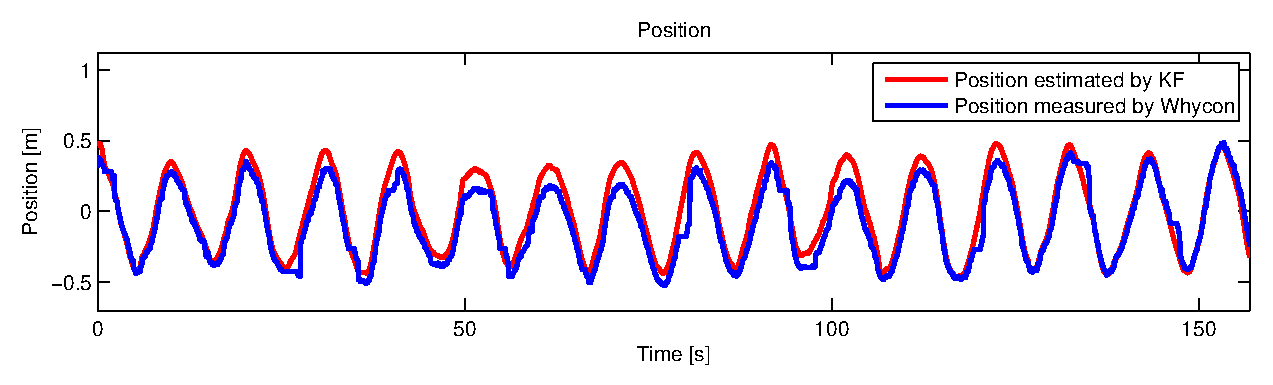
\includegraphics[width=0.99\textwidth]{fig/experiment5_drift_sine.eps}
\caption{Experiment with measuring position drift while tracking a sine trajectory (forward motion).}
\label{fig:experiment_drift_sine}
\end{figure}

\subsection{Tracking dynamic trajectory}
\label{cap:dynamic_trajectory_tracking}

Another experiment tested the system's capability of tracking dynamic trajectories. The first one tested the UAV to \emph{unit step} response. As it can be seen in figure \ref{fig:experiment_step}, the UAV does not overshoot the setpoint, but it rather makes a proaction which is a typical characteristic of the model predictive controller. The speed lies within the set boundaries due to input governor.

Figure \ref{fig:experiment_sine_1} shows the performance during tracking a circular trajectory. The trajectory was precomputed with constant speed $0.25\jed{ms^{-1}}$. Figure shows position and speed for both attitude axis. The experiment can bee seen in the compilation video which can be found at \url{http://youtu.be/lPy7w-GUbw4} or in the enclosed CD. The maximum deviation from the desired trajectory (forward motion) was $\Delta_{max} = 16.3\jed{cm}$, the standard deviation $\sigma = 4.3\jed{cm}$.

\begin{figure}[h]
\centering
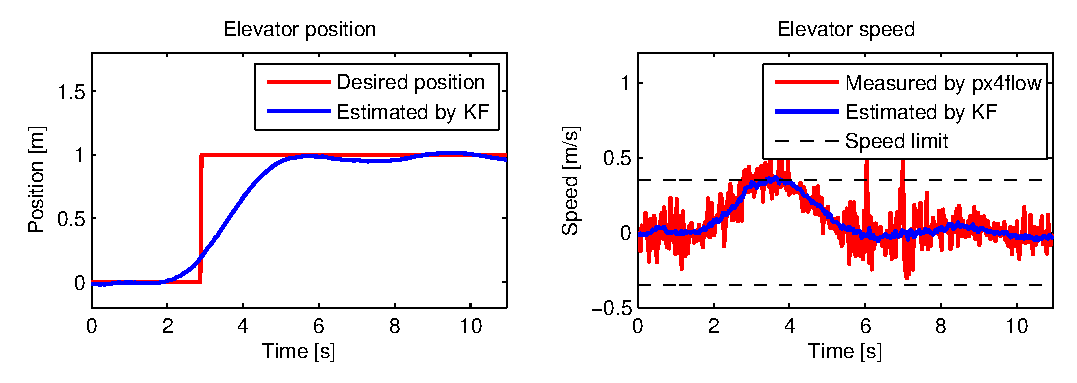
\includegraphics[width=0.99\textwidth]{fig/experiment2_step.eps}
\caption{Experiment with tracking the \emph{unit step} response.}
\label{fig:experiment_step}
\end{figure}

\begin{figure}[H]
\centering
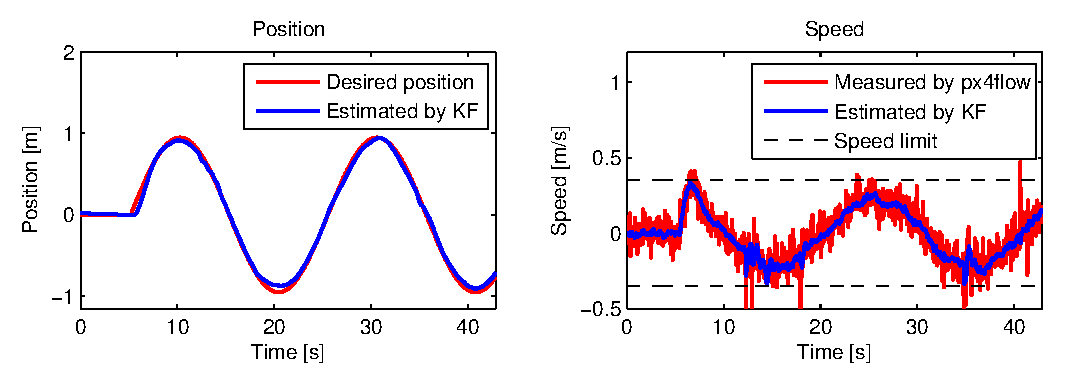
\includegraphics[width=0.99\textwidth]{fig/experiment1_sine.eps}
\caption{Experiment with tracking circular trajectory. Amplitude $0.95\jed{m}$, period $20\jed{s}$, speed $0.24\jed{ms^{-1}}$.}
\label{fig:experiment_sine_1}
\end{figure}

\subsection{Disturbance rejection}

\begin{figure}[b]
\centering
\includegraphics[width=0.7\textwidth]{fig/disturbance.jpg}
\caption{Experimental setup with $40\jed{W}$ fan to test the disturbance rejection feature.}
\label{fig:vetrak1}
\end{figure}

Experiments were also conducted to test the disturbance rejection capability. Since we dealt with the real hardware where the dynamical model is only its approximation, we cannot suppose the same performance during the experiments as it was observer during simulations. It was mostly observed during tuning of the disturbance estimator. By decreasing the settling time of the estimated disturbance, the system become unstable due to oscillations being induced into the estimate which led to worse performance. We found sufficient parameters that allow to estimate normal disturbances, such as bad trimming or stabilization offset, in order of seconds. 
 
\subsubsection{Persistent wind disturbances}
\label{cap:persistant_wind_disturbances_experiment}

The UAV was tested for its capability to reject wind disturbances by setting a $40\jed{W}$ fan pointed to the UAV (see figure \ref{fig:vetrak1}). To put into context, it is the same power as one of UAV's motors. The figure \ref{fig:experiment_steady_wind} shows the forward motion of the aircraft. The grey area indicates where the fan was turned on. The estimated disturbance settled in $\approx 10\jed{s}$ which allowed the UAV to eliminate the resulting \emph{steady state} error. Notice the non-zero disturbance when the fan is turned off --- caused by already mentioned trimming and stabilization offset.

\begin{figure}[h]
\centering
	\begin{tikzpicture}
		\node[anchor=south west,inner sep=0] (a) at (0,0) {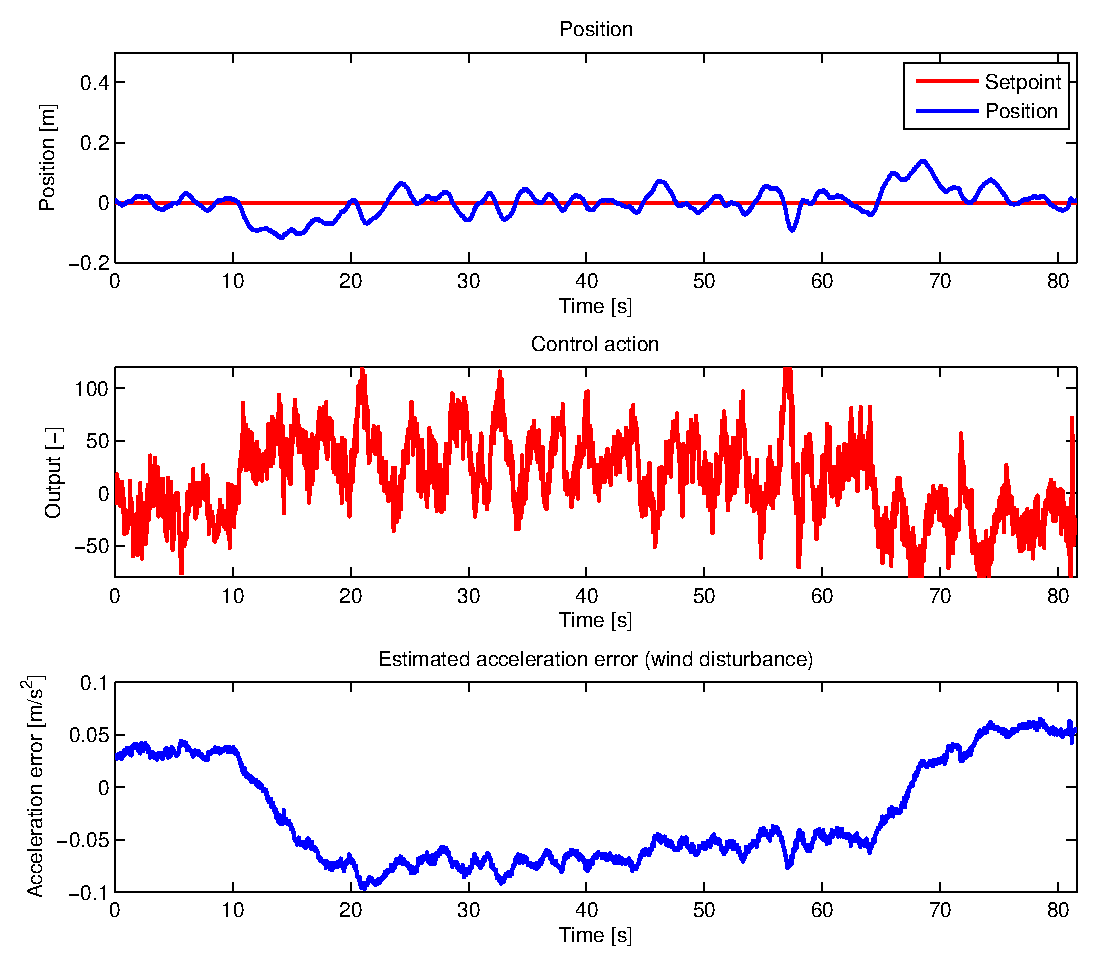
\includegraphics[width=\textwidth]{fig/experiment3_steady_disturbance.eps}};
		\begin{scope}[x={(a.south east)},y={(a.north west)}]

		%\draw[help lines,xstep=.1,ystep=.1] (0,0) grid (1,1);	
		
%        \draw[white,ultra thick,rounded corners] (0.55,0.50) rectangle (0.7,0.7);
%        \draw (0.58,0.655) node [text=white] {\textbf{1}};
        

		%\draw[-latex] (0.2,0.9) -- (0.2,0.81);    
		%\node[] at (0.25,0.92) {Disturbance started};    
		
		%\draw[-latex] (0.75,0.9) -- (0.795,0.81);    
		%\node[] at (0.65,0.92) {Disturbance went off};  
		
		\draw[fill=gray, opacity=0.2] (0.2,0.740) rectangle (0.757,0.960);  
		
		\draw[fill=gray, opacity=0.2] (0.2,0.401) rectangle (0.757,0.624);  
		
		\draw[fill=gray, opacity=0.2] (0.2,0.064) rectangle (0.757,0.286);  
        
    \end{scope}
	\end{tikzpicture}
\caption{Experiment with tracking constant setpoint while being under the influence of wind.}
\label{fig:experiment_steady_wind}
\end{figure}

\subsubsection{Momentary disturbances}
\label{cap:momentary_disturbances}

The final experiment aimed to test the capability of rejecting sudden disturbances. Figure \ref{fig:experiment_momentary_disturbances} shows a forward motion of experiment, that can be again seen in the compilation video. ZDE BUDE VÍC TEXTU

\begin{figure}[h]
\centering
	\begin{tikzpicture}
		\node[anchor=south west,inner sep=0] (a) at (0,0) {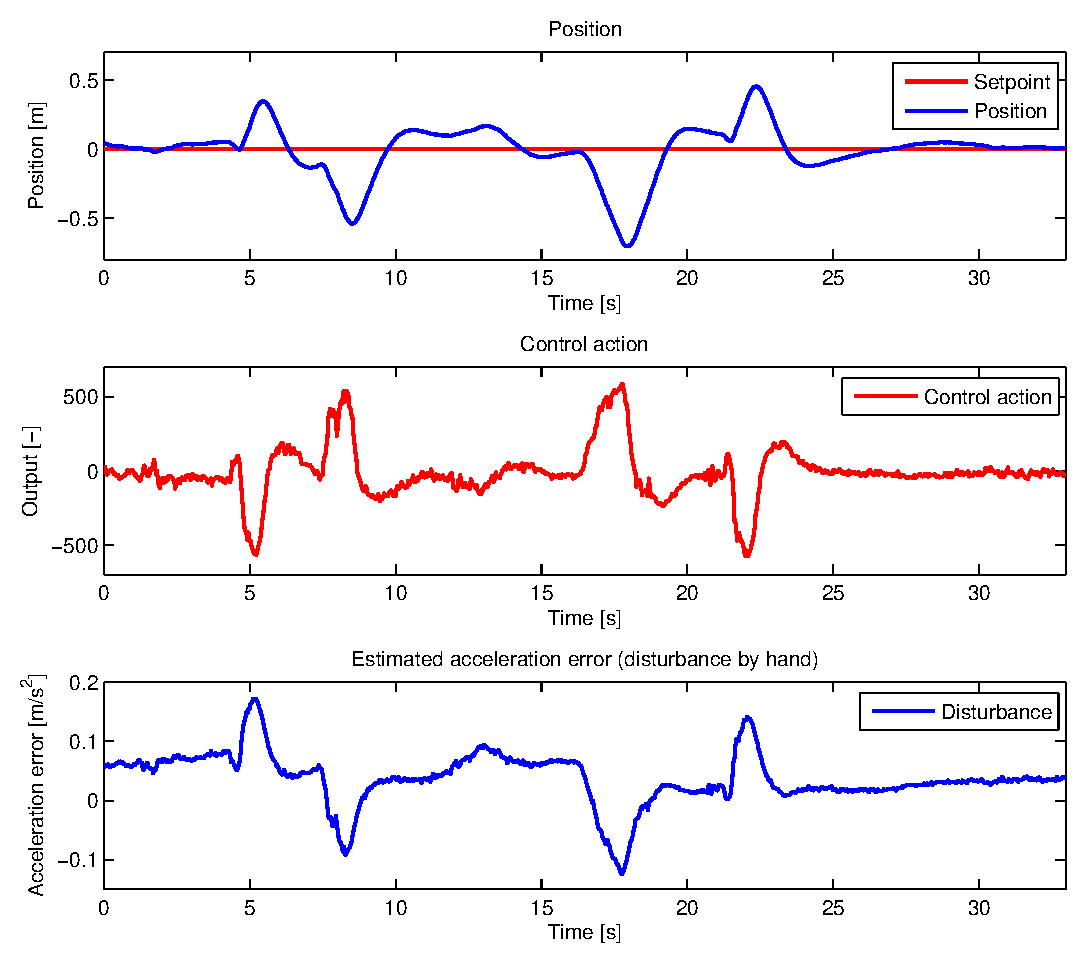
\includegraphics[width=\textwidth]{fig/experiment4_sudden_disturbances.eps}};
		\begin{scope}[x={(a.south east)},y={(a.north west)}]

%		\draw[help lines,xstep=.1,ystep=.1] (0,0) grid (1,1);	
		
%        \draw[white,ultra thick,rounded corners] (0.55,0.50) rectangle (0.7,0.7);
%        \draw (0.58,0.655) node [text=white] {\textbf{1}};

		\draw[fill=gray, opacity=0.2] (0.205,0.739) rectangle (0.235,0.9615);  
		\draw[fill=gray, opacity=0.2] (0.29,0.739) rectangle (0.319,0.9615);  
		\draw[fill=gray, opacity=0.2] (0.41,0.739) rectangle (0.445,0.9615);  
		\draw[fill=gray, opacity=0.2] (0.532,0.739) rectangle (0.575,0.9615);  
		\draw[fill=gray, opacity=0.2] (0.675,0.739) rectangle (0.7,0.9615); 
		
		\draw[fill=gray, opacity=0.2] (0.205,0.4015) rectangle (0.235,0.624);  
		\draw[fill=gray, opacity=0.2] (0.29,0.4015) rectangle (0.319,0.624);  
		\draw[fill=gray, opacity=0.2] (0.41,0.4015) rectangle (0.445,0.624);  
		\draw[fill=gray, opacity=0.2] (0.532,0.4015) rectangle (0.575,0.624);  
		\draw[fill=gray, opacity=0.2] (0.675,0.4015) rectangle (0.7,0.624); 
		
		\draw[fill=gray, opacity=0.2] (0.205,0.063) rectangle (0.235,0.286);  
		\draw[fill=gray, opacity=0.2] (0.29,0.063) rectangle (0.319,0.286);  
		\draw[fill=gray, opacity=0.2] (0.41,0.063) rectangle (0.445,0.286);  
		\draw[fill=gray, opacity=0.2] (0.532,0.063) rectangle (0.575,0.286);  
		\draw[fill=gray, opacity=0.2] (0.675,0.063) rectangle (0.7,0.286); 
        
    \end{scope}
	\end{tikzpicture}
\caption{Experiment with tracking constant setpoint while being under the influence of momentary disturbances. The UAV was dragged by hand which is indicated by the gray areas.}
\label{fig:experiment_momentary_disturbances}
\end{figure}

\subsection{Summary and comparison with previous work}

Je to krásné, létá to!!!